%%%%%%%%%%%%%%%%%%%%%%%%%%%%%%%%%
% Space complexity
%%%%%%%%%%%%%%%%%%%%%%%%%%%%%%%%%
\section{Space complexity}
\label{sec:space_comp}

If the finite cardinality of a universe is $u$ and the set is \emph{dense} (and the approximation is also dense, i.e., the false negative rate is relatively
small), then
\begin{equation}
    \mathcal{O}(u) \; \si{bits}
\end{equation}
suffice to code the set (an exact bit vector), which is independent of $\p$, the false positive rate, and the false negative rate.

The lower-bound on the \emph{expected} space complexity of a data structure that models the \emph{positive random approximate set} where the elements are over a \emph{countably infinite} universe is a classical result due to Carter, Floyd, Gill, Markowsky, and Wegman~\cite{carterExact}.
We restate it here in the notation of the present paper and include a proof for completeness.
\begin{proposition}[{\cite{carterExact}}]
\label{pst:approx_l_b}
The \emph{information-theoretic lower-bound} of a data structure that implements the countably infinite \emph{positive random approximate set} abstract data type has an \emph{expected} bit length given by
\begin{equation}
    -\log_2 \fprate \; \si{bits \per element},
\end{equation}
where $\fprate > 0$ is the false positive rate.
\end{proposition}
\begin{proof}
We give the counting argument for deterministic fixed-length encodings.
The extension to randomized structures is the standard averaging argument
behind Yao's principle~\cite{yaoMinimax}, sketched here and not claimed as new.
Draw $S$ uniformly from the size-$\p$ subsets and regard a randomized structure
as a distribution over deterministic encodings indexed by its seed $R$.
Given $R$ and the encoded state, $S$ is a size-$\p$ subset of the positive
response set, so its conditional entropy is at most the expectation of
$\log_2\binom{\p + x(n-\p)}{\p}$, where $x$ is the realized fraction of
negatives accepted.
That function is concave in $x$ and $\Expect{x} \leq \fprate$, so by Jensen's
inequality the bound below holds with $B$ read as the expected length of a
prefix-free encoding, which is at least the entropy of the encoded state.


Consider a finite subset of the universe with $n$ elements, from which an
objective set $S$ of size $\p$ is drawn.
A deterministic encoding using $B$ bits maps each input set $S$ to a state
$r = f(S)$ from at most $2^B$ distinct states.
Each state $r$ determines a \emph{positive response set}
$Q(r) = \{x : \text{query}(x,r) = 1\}$.
Since the data structure has no false negatives ($\tprate = 1$), we have
$S \subseteq Q(r)$ for the state $r = f(S)$ encoding $S$.
The false positive rate constraint requires that at most an $\fprate$-fraction of the $n - \p$ negatives belong to $Q(f(S))$ for every input set $S$, so
$|Q(f(S))| \leq \p + \fprate(n - \p)$ for all $S$.
In particular, $|Q(r)| \leq \p + \fprate(n - \p)$ for every state $r$ in the image of $f$.

By the pigeonhole principle, some state $r^*$ must encode at least
$\binom{n}{\p} / 2^B$ distinct input sets.
Every such set is a subset of $Q(r^*)$ of size $\p$, so
\begin{equation}
\binom{n}{\p} / 2^B
    \leq \binom{|Q(r^*)|}{\p}
    \leq \binom{\p + \fprate(n - \p)}{\p}.
\end{equation}
Taking logarithms and rearranging:
\begin{equation}
B \geq \log_2 \binom{n}{\p} - \log_2 \binom{\p + \fprate(n - \p)}{\p}.
\end{equation}
For fixed $\p$ as $n \to \infty$, $\binom{n}{\p} \sim n^\p / \p!$ and
$\binom{\p + \fprate n}{\p} \sim (\fprate n)^\p / \p!$, so the right-hand side increases to
$\log_2 \bigl(n^\p / (\fprate n)^\p\bigr) = -\p \log_2 \fprate$ from below and
\begin{equation}
B \geq -\p \log_2 \fprate - o(1) \qquad (n \to \infty),
\end{equation}
giving $-\log_2 \fprate$ bits per element in the countably infinite limit.
This is a fixed-size, growing-universe regime, unlike the constant-density
regime of \cref{thm:joint_entropy_fp_fn}.
\end{proof}
\begin{remark}[The two-sided case]
\label{rem:general_lower_bound}
When false negatives occur ($0 < \tprate < 1$), $S \not\subseteq Q(r)$ and the
pigeonhole step above does not apply directly.
An earlier version of this preprint called this case open; it is not.
Pagh and Rodler~\cite[Prop.~1]{paghRodlerLossy} show that a lossy dictionary
storing $n$ keys from a universe of size $2^w$, with at most $\gamma n$ false
negatives and false positive rate $\fprate$, needs at least
$(1-\gamma)\, n \log_2\bigl(1/(\fprate + n/2^w)\bigr) - \mathcal{O}(n)$ bits.
In the large-universe limit, with $\gamma = 1 - \tprate$, this is
$-\tprate \log_2 \fprate - \mathcal{O}(1)$ bits per element, so the scaling
$-\tprate \log_2 \fprate$ (retaining $\p \tprate$ elements, each costing
$-\log_2 \fprate$ bits) is a valid lower bound up to an additive constant per
element.
Their model bounds the number of false negatives, whereas the Bernoulli model
fixes their expected rate; we do not carry out that transfer here.
\end{remark}

A well-known implementation of countably infinite \emph{positive approximate set} is the Bloom filter~\cite{bf} which has an expected space complexity given
by~\cite{broderMitzenmacher}
\begin{equation}
    -\frac{1}{\ln 2} \log_2 \fprate \; \si{bits \per element},
\end{equation}
thus the absolute efficiency of the Bloom filter is $\ln 2 \approx 0.69$.
Constructions that meet the bound of \cref{pst:approx_l_b} up to
lower-order terms are known~\cite{paghPaghRao,dietzfelbingerPagh}.
A practical implementation of the \emph{positive random approximate set} is given by the \emph{Perfect Hash Filter}~\cite{phf}, a minimal perfect hash function that stores a $\log_2(1/\fprate)$-bit fingerprint per element, as described by Dietzfelbinger and Pagh~\cite[Sec.~1]{dietzfelbingerPagh}; it compares favorably to the Bloom filter in many circumstances.\footnote{The \emph{Bernoulli hash function}~\cite{shs} (earlier called the singular hash set) attains the bound by \emph{brute-force} search for a seed, so it is not practical for even relatively small objective sets; its purpose is analytic tractability. Single-seed search of this kind, with storage near the information scale and exponential construction work, is analyzed by Lehmann et al.~\cite{lehmannSeeds}.}

\begin{figure}[ht]
\centering
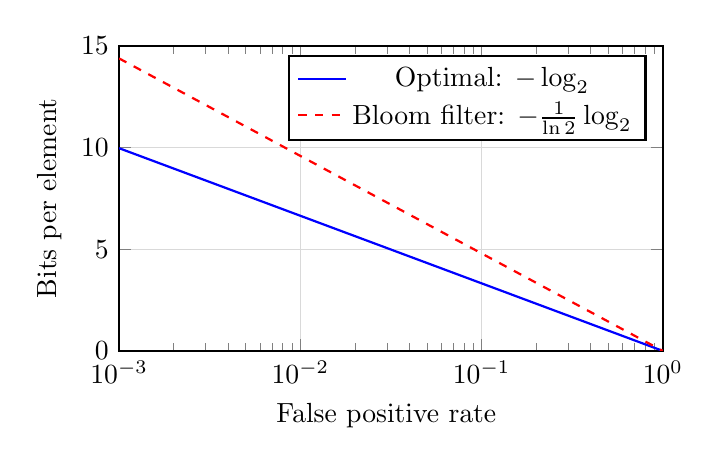
\begin{tikzpicture}
\begin{axis}[
	width=0.7\textwidth,
	height=0.45\textwidth,
	xlabel={False positive rate $\fprate$},
	ylabel={Bits per element},
	xmin=0.001, xmax=1,
	ymin=0, ymax=15,
	xmode=log,
	legend pos=north east,
	ymajorgrids, xmajorgrids,
	major grid style={gray!30},
	thick,
	samples=200,
	domain=0.001:1,
]
\addplot[blue, solid] {-ln(x)/ln(2)};
\addlegendentry{Optimal: $-\log_2 \fprate$}
\addplot[red, dashed] {-ln(x)/ln(2)/ln(2)};
\addlegendentry{Bloom filter: $-\frac{1}{\ln 2}\log_2 \fprate$}
\end{axis}
\end{tikzpicture}
\caption{Space complexity of positive approximate sets as a function of
the false positive rate $\fprate$.
The solid curve is the information-theoretic lower bound
$-\log_2 \fprate$ bits per element (\cref{pst:approx_l_b}).
The dashed curve is the Bloom filter cost
$-(1/\ln 2)\log_2 \fprate$; the gap reflects the Bloom filter's
$\ln 2 \approx 69\%$ efficiency.}
\label{fig:space_lower_bound}
\end{figure}
